\documentclass[runningheads]{llncs}

\usepackage{graphicx}
\graphicspath{{./figs/}}

\usepackage{amsmath} 
\usepackage{bm}
\usepackage{amsbsy} 
\usepackage{amssymb}
\usepackage{cite}

\begin{document}
%
\title{Multiscale model reduction for neutron diffusion equation}
%
%\titlerunning{Abbreviated paper title}
% If the paper title is too long for the running head, you can set
% an abbreviated paper title here
%
\author{A.O. Vasilev\inst{1} \and 
D.A. Spiridonov\inst{1} \and
A.V. Avvakumov\inst{2} }
%
\authorrunning{A.O. Vasilev, D.A. Spiridonov \and A.V. Avvakumov}
% First names are abbreviated in the running head.
% If there are more than two authors, 'et al.' is used.
%
\institute{North-Eastern Federal University, Yakutsk, Russia \and
National Research Center \emph{Kurchatov Institute}, Moscow, Russia\\
\email{haska87@gmail.com}
}
%
\maketitle              % typeset the header of the contribution
%
\begin{abstract}
Construction of multiscale method for neutron diffusion equation is provided. 
The neutron diffusion approximation is mostly used for reactor analysis and applied in most engineering calculation codes. 
The solution method is based on the use of a generalized multiscale finite element method.
The main idea is to create local solutions that can be used to effectively solve on a coarse grid.
Numerical results show that multiscale basis functions can well take into account the small-scale characteristics of the medium and provide accurate solutions. 

\keywords{multiscale method \and parabolic equation \and neutron diffusion}
\end{abstract}

\section{Introduction}
About neutron diffusion equation \\
bla bla bla \\
bla bla bla \\
bla bla bla \\
bla bla bla \\
About reduction methods \\
bla bla bla \\
bla bla bla \\
bla bla bla \\
bla bla bla \\
bla bla bla \\
About GMsFEM method \\
bla bla bla \\
bla bla bla \\
bla bla bla \\
bla bla bla \\
About results \\
bla bla bla \\
bla bla bla \\
bla bla bla \\

\section{Problem statement}
Let's consider modelling neutron flux in a one-group diffusion approximation. 
Neutron flux dynamics is considered within a bounded 2D domain  $\Omega$ ($\bm x = \{x_1, x_2\} \in \Omega$) with a convex boundary $\partial \Omega$. 
The neutron diffusion is described by the following set of equations with one group delayed neutron source:
\begin{equation}\label{1}
\begin{split}
 \frac{1}{v} \frac{\partial \phi}{\partial t} - \nabla \cdot D \nabla \phi + \Sigma_r \phi &= \frac{1 - \beta}{K_{eff}} \nu \Sigma_f \phi + \lambda c, \\
\frac{\partial c}{\partial t} + \lambda c &= \frac{\beta}{K_{eff}} \nu \Sigma_f \phi.
\end{split}
\end{equation} 
Here $\phi(\bm x,t)$ --- neutron flux  at point $\bm x$ and time $t$,
$v$ --- effective velocity of neutrons,
$D(\bm x)$ --- diffusion coefficient, 
$\Sigma_r(\bm x,t)$ --- removal cross-section,
$\Sigma_f(\bm x,t)$ --- generation cross-section,
$\beta$ --- effective fraction of delayed neutrons, 
$\lambda$ --- decay constant of sources of delayed neutrons.
System of equations (\ref{1}) is supplement with boundary condition and  initial condition.

The albedo-type conditions are set at the boundary of the area $\partial \Omega$:
\begin{equation}\label{2}
 D\frac{\partial \phi}{\partial n} + \gamma \phi = 0,
\end{equation} 
where $n$ --- outer normal to the boundary $\partial \Omega$, $\gamma$ --- albedo constant.
Let's propose that in the initial time moment (at t = 0) the reactor is in the critical state
\begin{equation}\label{3}
 \phi(\bm x,0) = \phi^0(\bm x).
\end{equation} 
%Let's consider problem (\ref{1}) with boundary conditions (\ref{2}) and initial conditions

To solve the problem in computational domain $\Omega$, we approximate the system of equations (\ref1)-(\ref{3}) using the finite element method.
We discretize the time derivatives using finite-difference scheme, and then bring each stationary problem to a variational formulation. 
For approximation in time, we use a purely implicit scheme with time step $\tau$. 
To specify the variational formulation, we multiply equations by the test function $q$ and integrate over the domain $\Omega$. 
Using the integration by parts, we obtain the following variational formulation: find $\phi^{n+1} \in V$ such that
\begin{equation} \label{4}
\begin{split}
\int_\Omega \frac{1}{v} \frac{\phi^{n+1}}{\tau} q dx +
\int_\Omega D^{n+1} \nabla\phi^{n+1} \cdot \nabla q dx &+ 
\int_\Omega \Sigma_r^{n+1} \phi^{n+1} q dx - \\
\int_\Omega \frac{1+\lambda\tau-\beta}{K_{eff}(1+\lambda\tau)} \nu \Sigma_f^{n+1} \phi^{n+1} q dx &+
\int_{\partial \Omega} \gamma \phi^{n+1} q ds = \\
\int_\Omega \frac{1}{v} \frac{\phi^{n}}{\tau} q dx +
\int_\Omega \frac{\lambda c^n}{1+\lambda\tau} q dx &, \quad \forall q \in V,
\end{split}
\end{equation}
where $V=H^1(\Omega)$ --- sobolev space consisting of scalar functions $\upsilon$ such that $\upsilon^2$ and $|\nabla \upsilon^2|$ have a finite integral in $\Omega$.

Further, it's necessary to pass from the continuous variational problem (\ref{4}) to the discrete problem. 
We introduce finite-dimensional space of finite elements $V_h \subset V$ and formulate a discrete variational problem. 
We use standard linear basis functions as basis functions to solve the problem on the fine grid and
\[
\phi = \sum_{i = 1}^{N_f} \phi_i y_i,
\] 
where $N_f$ is the nunber of vertices on the fine grid.

The problem is solving a system of linear algebraic equations
\begin{equation}\label{5}
A\phi = b,
\end{equation}
where the operator $A$ corresponds to the left side of equation (\ref{4}), and the vector $b$ corresponds to the right side of equation (\ref{4}).

\section{Multiscale method}
For the discretization on the coarse grid we use GMsFEM.
We construct two grids: fine grid ($\mathcal{T}_h$) and coarse grid ($\mathcal{T}_H$) (see Figure \ref{p1}). 
For multiscale basis construction, we define local domains $\omega_i$, where $i = 1,...,N_v$ and $N_v$ is the number of coarse grid nodes.
We assume that $\mathcal{T}_h$ is a refinement of $\mathcal{T}_H$, where $h$ and $H$ represent the fine and coarse mesh sizes, respectively. 
We assume that the fine-scale mesh $\mathcal{T}_h$ is sufficiently fine to fully resolve the small-scale information of the domain  while $\mathcal{T}_H$ is a coarse mesh containing many fine-scale features.
A local domain $\omega_i$ is obtained by the combining all the coarse cells around one vertex of the coarse grid. 
%The number of such domains will be equal to the number of vertices of our coarse grid.  
%In Figure \ref{p1} we present local domain $\omega _i$.
%For multiscale In such coarse subdomains $\omega _i$ we will solve local problems to construct a multiscale space. 
%We construct a multiscale basis functions in each local domain by the solution of the local spectral problem that help to select important modes of the solution.

\begin{figure}[h!]
\centering

\includegraphics[width=0.26\linewidth]{coarse_grid.png}
\hspace{2em}
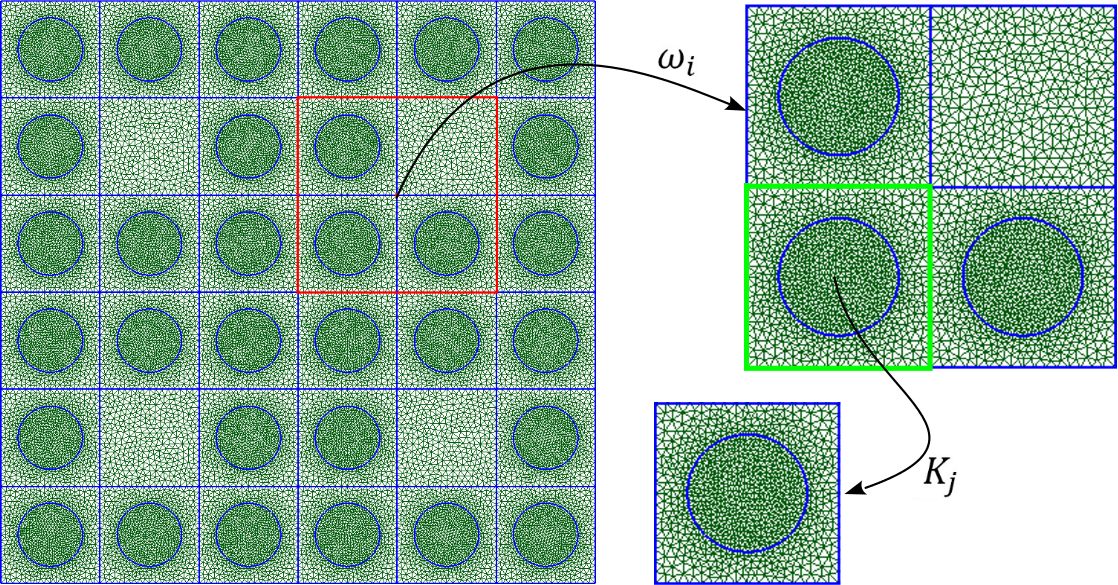
\includegraphics[width=0.5\linewidth]{omega.png} 
\caption{Coarse grid and local domain $\omega_i$ with $K_j$}
\label{p1}
\end{figure} 

GMsFEM  involves two basic steps: (1) the construction of multiscale basic functions that take into account small scale heterogeneities in the local domains and (2) the construction of the coarse scale approximation. 
For the construction of the multiscale basic functions we solve spectral problems in local domains.
Spectral problems help to identify the most important characteristics of the solution. 
In contrast to the available techniques, this method allows to avoid the limitations associated with idealization and limitations on the applicability of the method.
This method also more general technology that takes into account the different scale processes.
The construction of basic functions occurs independently for each local domain, doesn't require the exchange of information between processors, and  has a high parallelization efficiency.
Using constructed multiscale basic functions, we construct a mathematical model on a coarse grid that allows to significant reduce the solution time, the amount of used memory, and can be used to perform calculations for a given configuration of  heterogeneous properties.

%\subsection{Multiscale Basis Funtions}
We construct the mutiscale function space
\[
{V}_{\text{off}} = \mbox{span} \{ y_j \}_{j=1}^{N},
\]
where $N$ is the number of coarse basis functions.
Each $y_j$ is supported in local domain $w_i$.

% spectral
\textbf{Multiscale space.}
The firts step is the solution of local spectral problems on the local domains. These spectral problems identify important modes of the problem and used to construct a multiscale space. In order to construct a conforming basis functions, we multiply eigenvectors related to the smallest eigenvalues to the partition of unity functions.
 
We use following spectral problem in $\omega_i$
\begin{equation} \label{e4}
A \varphi^i = \lambda S \varphi^i,
\end{equation} 
where the elements of the matrices $A= \{ a_{ij} \}$ and $S = \{ s_{ij} \}$ are defined as follow{
\begin{equation} \label{e5}
\begin{split}
a_{ij} = 
\int_{\omega_i} D \nabla\phi \cdot \nabla q dx &+ 
\int_{\omega_i} \Sigma_r \phi q dx - 
\int_{\omega_i} \frac{1+\lambda\tau-\beta}{K_{eff}(1+\lambda\tau)} \nu \Sigma_f \phi q dx, \\
s_{ij} &= \int_{\omega _i} D u q dx.
\end{split}
\end{equation}}
We solve this spectral problem on the local domain
\begin{equation} \label{e8}
\tilde{A} \tilde{\varphi}^i = \lambda \tilde{S}  \tilde{\varphi}^i, \quad
\tilde{A} = P A P^T, \quad \text{ and } \quad 
\tilde{S} = P S P^T.
\end{equation}
where $P = \{ \psi_0, \psi_1, ...,\psi_{J_i} \}$ and {$\varphi^i_k = P \tilde{\varphi}^i_k$} for $k = 1,2,...$.
{Then, we choose eigenvectors corresponding to the smallest $M_{i}$ eigenvalues from \eqref{e8} and use them for the construction of multiscale basis functions.} 
%In Figure \ref{p6}, we present first four eigenvectors. 

% POU
\textbf{Partirion of unity functions. } As  partition of unity functions, we use linear functions in each domain $\omega_i$.
Partitions of unity are calculated in the domain $ K_j $ as a linear function from $\Gamma$ to the vertex $ A $, and $ 0 $ is assigned to the entire segment $\Gamma$, and at point $ A $ is assigned the value $1$. 
Thus, we obtain a linear function from $ 0 $ to $ 1 $ over the entire domain $ K_j $. 
Partitions of unity are shown in Figure \ref{p2}. 
Domain $K_j$  is one element from a coarse grid. 

\begin{figure}[h!]
\centering
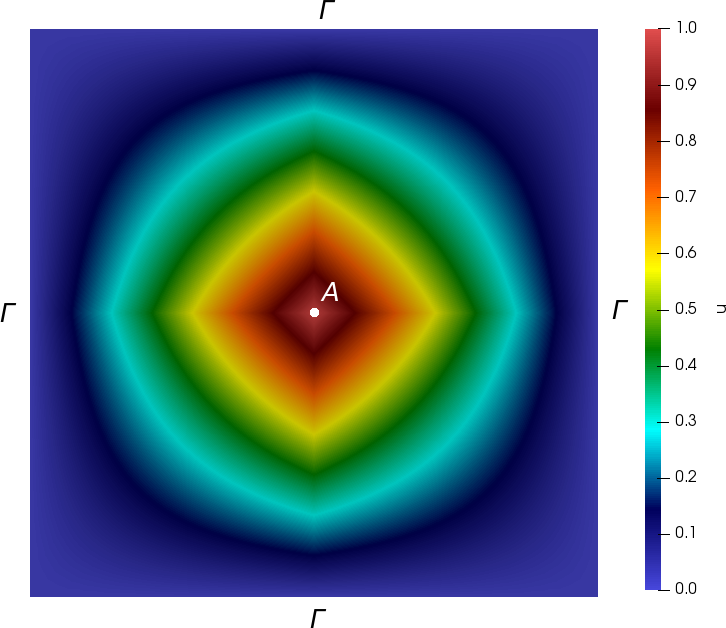
\includegraphics[width=0.4\linewidth]{pofs.png} 
\hspace{2em}
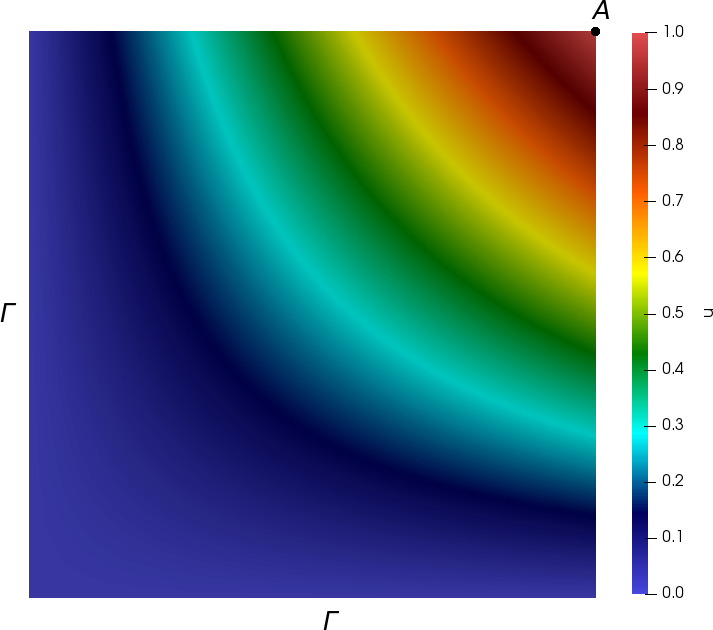
\includegraphics[width=0.4\linewidth]{pouK.png} 
\caption{Partirion of unity functions on the $\omega_i$ (right) and $K_j$ (left)}
\label{p2}
\end{figure} 
 
The multiscale space is defined as the span of $\chi_i \varphi^i_k$, where $\chi_i$ is the usual nodal basis function for the node $i$ (linear partition of unity functions). 
The number of bases can be different, the accuracy of the solution can be improved when we increase the number of bases.
%In Figure \ref{p7}, we present first four multiscale basis functions in local domain $\omega_i$.

%\subsection{Assembling a matrix in a multiscale space}
\textbf{Coarse-scale approximation. }
Next, we create following  matrix for each $\omega_i$
\[
R^i = \left[ \chi_i \varphi_1^i, \ldots, \chi_i \varphi_{M_i}^i,  \chi_i \eta^i \right].
\]
and  define a transition matrix from a fine grid to a coarse grid to reduce the dimension of the problem
\[
R = [ R^1, R^2, ..., R^{N_v} ],
\]
where $N_v$ is the number of local domains $\omega_i$.

Then using transition matrix $R$ and fine grid system  \ref{5}, we construct coarse grid approximation
\begin{equation}\label{e12}
A_c \phi_c = b_c, \quad 
A_c = R A R^T 
\quad \text{ and } \quad 
b_c = R b,
\end{equation}  
and using coarse-scale solution $\phi_c$, we can  reconstruct a fine grid solution $\phi_{ms} = R^T \phi_c$.

\section{Numerical results}


\section*{Acknowledgements}
This work was supported by the grant of the Russian Federation Government
(\#14.Y26.31.0013) and the Russian Science Foundation (\#19-71-00008).

\begin{thebibliography}{8}
\bibitem{Annals17}
Avvakumov,~A.~V., et al.: Spectral properties of dynamic processes in a nuclear reactor. Annals of Nuclear Energy. \textbf{99}, 68--79 (2017) 

\bibitem{Progress18}
Avvakumov A. V. et al.: State change modal method for numerical simulation of dynamic processes in a nuclear reactor. Progress in Nuclear Energy. \textbf{106}, 240--261 (2018)

\end{thebibliography}
\end{document}
